\Chapter{Elméleti háttér}

Szakdolgozatom célja létrehozni egy olyan kliens-szerver weboldalt, amely bárki számára könnyen használható és látványok kimutatásokat tud ezáltal készíteni. Már a tervezési fázisban elhatároztam, hogy a weboldal felépítése hasonlítani fog a kutatásom során megismert tőszdei témájú weboldalakhoz, mind felépítésében, mind megvalósításában, hogy a felhasználó azt érezze egy\textit{ élő és lélegző weboldal}on böngészik. Ehhez viszont előtte szeretném ismertetni a szakdolgozatomhoz szükséges tudáshátteret.

\Section{Grafikonok története}

Egy látványos grafikonnal könnyebb bemutatni egy elemzést, vagy történetet, mint szóban elmesélni. Ugyan ma alapkellékként értelmezzük vonaldiagramokat és kördiagramokat, viszont egykor forradalmi újításnak Számítottak. Volt rá példa, hogy használatuk szó szerint életbevágónak bizonyult. Amikor egy angol orvosnő, Florence Nightingale, diagramok segítségével győzte meg a 19. századi férfiak által vezetett orvosok közösségét, hogy jobban oda kéne figyelniük a kórházi higiéniára. A kifogástalan és figyelem felkeltő grafikonjának hála, katonák tömegei élték túl a krími háborút.  \cite{portfolio}

	A grafikon a diagram egyik fajtája, amely két adat kapcsolatát egy derékszögű koordináta-rendszerben ábrázolja. A két tengely jelképezi a két adatot, és a grafikon jelzi, hogy az egyik adatnak az egyes értékeihez a másik mely értékei tartoznak. Általában két mennyiség közötti lineáris kapcsolatot, vagy egy mennyiség időbeli változásának bemutatására használják. Matematikai szemszögből a grafikon egy függvényt ábrázol. \cite{wikiMatek}

\begin{figure}[h]
\centering
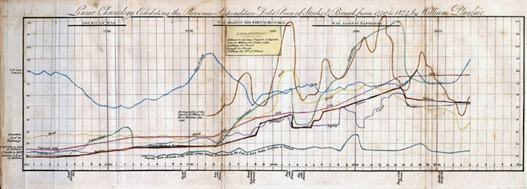
\includegraphics[scale=0.5]{images/historyOfGraphs}
\caption{Az egyik első statisztikai gráf (forrás: \cite{oldGraph})}
\end{figure}

\Section{Tőzsde}

A tőzsde talán a modern világ egyik legjobban félreértelmezett kifejezése, amire egy hétköznapi személy csak legyint, hogy úgy se értené meg és ez csak az egész nap monitort figyelő brókereknek való. Nos ez az állítás részben igaz is, hiszen lehet nagyon bonyolult a tőzsde, viszont lehet nagyon egyszerű is.
	A tőzsde egy olyan nyilvános, központosított és szervezett piac, ahol meghatározott árukat, meghatározott időben, azon belül meghatározott személyek adhatnak, vagy vehetnek szigorú eljárási szabályok szerint.  Hogy ez mit is jelent a gyakorlatban? A tőzsde is egy olyan piac, mint akármelyik városban, vagy faluban találhatunk. A különbség az, hogy vásárlás során maga az áru nem materiális formában jelenik meg, illetve nem csak az adott környezettel, hanem az egész világgal lehetőségünk van kereskedni. Viszont, hogy mibe érdemes fektetni az bonyolultabb, mint elsőre képzelnénk. 
\begin{itemize}
\item Irodalomkutatás. Amennyiben a dolgozat egy módszer kidolgozására, kifejlesztésére irányul, akkor itt lehet részletesen végignézni (módszertani vagy időrendi bontásban), hogy az eddigiekben milyen eredmények születtek a témakörben.
\item Technológia. Mivel jellemzően kutatásról vagy szoftverfejlesztésről van szó, ezért annak a jellemző elemeit, technikai részleteit itt kell bemutatni.
Ez tehát egy módszeres bevezetés ahhoz, hogy ha valaki nem jártas a témakörben, akkor tudja, hogy a dolgozat milyen aktuálisan elérhető eredményeket, eszközöket használt fel.
\item Piackutatás. Bizonyos témáknál új termék vagy szolgáltatás kifejlesztése a cél.
Ekkor érdemes annak alaposan utánanézni, hogy aktuálisan milyen eszközök érhetők el a piacon.
Ez szoftverek esetében a hasonló alkalmazások bemutatását, táblázatos formában történő összehasonlítását jelentheti.
Szerepelhetnek képek és észrevételek a viszonyításként bemutatott alkalmazásokhoz.
\item Követelmény specifikáció. Külön szakaszban érdemes részletesen kitérni az elkészítendő alkalmazással kapcsolatos követelményekre.
Ehhez tartozhatnak forgatókönyvek (\textit{scenario}-k).
A szemléletesség kedvéért lehet hozzájuk képernyőkép vázlatokat is készíteni, vagy a használati eseteket más módon szemléltetni.
\end{itemize}

\Section{Amit csak említés szintjén érdemes szerepeltetni}

Az olvasóról annyit feltételezhetünk, hogy programozásban valamilyen szinten járatos, és a matematikai alapfogalmakkal sem ebben a dolgozatban kell megismertetni.
A speciális eszközök, programozási nyelvek, matematikai módszerekk és jelölések persze jó, hogy ha említésre kerülnek, de nem kell nagyon belemenni a közismertnek tekinthető dolgokba.
